\documentclass[conference]{IEEEtran}
\setlength{\columnsep}{0.21in}
\usepackage{amsmath,amsfonts,amssymb}
\usepackage{array}
\usepackage{textcomp}
\usepackage{stfloats}
\usepackage{url}
\usepackage{verbatim}
\usepackage{graphicx}
\usepackage[caption=false,font=footnotesize]{subfig}
\usepackage{tabularx}
\usepackage{gensymb}  
\usepackage{enumitem}
\usepackage{booktabs}
\usepackage{algorithm}
\usepackage{algpseudocode}  
\usepackage{xfrac}
%\usepackage[colorlinks=true, linkcolor=blue, citecolor=blue, urlcolor=blue]{hyperref}
\usepackage{cite}
\usepackage{lipsum}
\usepackage{multirow}
\usepackage{comment}
\usepackage{xcolor}

\title{Experimental Validation of Model-Based 3D Optical Wireless Positioning Using a Single Beam-Steered LED}
\author{
\IEEEauthorblockN{ Kevin Acuna-Condori*, Bastien Béchadergue*, Hongyu Guan*, and Luc Chassagne*}
\IEEEauthorblockA{ *Laboratoire d’Ingénierie des Systèmes de Versailles \\
                    Université Paris-Saclay, UVSQ, 78140 Vélizy-Villacoublay, France \\
                    Email: \{kevin-jose.acuna-condori, bastien.bechadergue, hongyu.guan, luc.chassagne\}@uvsq.fr}}

\begin{document}
\bstctlcite{IEEEexample:BSTcontrol}
\maketitle

\begin{abstract}
This paper presents the first experimental validation of three-dimensional (3D) optical wireless positioning based on a single beam-steered LED (SBL) and a single photodiode (PD) receiver. The method builds on a ratio-based formulation in which a single LED is successively steered toward $K=9$ different directions. Inter-orientation received signal strength (RSS) ratios are then formed to cancel the unknown receiver-orientation term, enabling two closed-form estimators, namely generalized least squares (GLS) and weighted least squares (WLS), to retrieve both the transmitter-to-receiver direction and the 3D receiver coordinates. The experimental campaign was conducted on a 3D testbed comprising a commercial infrared LED mounted on a two-axis motorized gimbal and a PD. The results show that the SBL principle is experimentally feasible in 3D with a minimal receiver architecture, and that GLS consistently outperforms WLS. For 3D positioning, GLS achieves a mean absolute error (MAE) of $9.97$ cm, compared with $11.98$ cm for WLS. For direction finding, GLS yields a pointing-error MAE of $4.06^\circ$, against $4.87^\circ$ with WLS, confirming its superior robustness, especially at large off-axis inclinations. 
\textcolor{blue}{Finally, an integration-time analysis shows that the median localization error remains essentially stable over a wide range of averaging windows, while the dispersion of the estimates decreases with modest temporal averaging.}
Overall, the results validate the practical viability of 3D SBL positioning and highlight its relevance for beam-aware indoor optical wireless communication.
\end{abstract}

\begin{IEEEkeywords}
3D indoor localization, beam steering, optical wireless positioning, visible light positioning.
\end{IEEEkeywords}



% =======================================================
\section{Introduction}
\label{sec:intro}
% =======================================================

Indoor positioning is a key enabler for emerging applications such as robotics, asset tracking, navigation, and context-aware wireless services. In this context, visible light positioning (VLP), and more broadly optical wireless positioning (OWP), have attracted significant interest because they can exploit LED-based infrastructure while offering high spatial reuse, low electromagnetic interference, and direct integration with optical wireless communication (OWC) systems \cite{Zhuang2018,Wang2024}. In particular, photodiode (PD)-based VLP remains attractive for practical deployment due to its low hardware complexity and high sampling capability. However, most PD-based VLP systems still follow a multi-anchor paradigm, in which several ceiling luminaires must be simultaneously visible to the user in order to enable robust positioning \cite{Bakar2021}. 
This requirement increases installation and calibration complexity and may also 
reduce effective coverage in sparsely lit areas or under restrictive field-of-view limits that hinder simultaneous multi-anchor visibility, 
thereby motivating architectures that can reduce the dependence on dense transmitter deployments.



To mitigate infrastructure density, recent research has increasingly investigated single-LED positioning \cite{Zhang2017,Hou2016,Li2023,Yu2018,Kim2022,Tran2022}. Existing single-LED demonstrations typically obtain the missing geometric degrees of freedom by increasing receiver-side capability, e.g., using image sensors and projective geometry \cite{Zhang2017,Hou2016,Li2023}, employing multi-PD receivers with tilted elements \cite{Yu2018}, or introducing receiver rotation, tracking, and/or learning-based inference \cite{Kim2022,Tran2022}. 
While these approaches validate the feasibility of single-LED localization, they often shift complexity to the user equipment (UE), through camera sensing, inertial aiding, mechanical actuation, or data-driven training pipelines, which may reduce interpretability and complicate generalization across devices and environments \cite{Tran2022}. 

In parallel, optical beam steering is becoming a core enabler in indoor OWC, supporting high-capacity links, dynamic beam management, and localization functionalities based on controlled beam scanning \cite{Koonen2021}. 
This naturally suggests a different architectural path for single-LED positioning: instead of increasing UE complexity, diversity can be generated at the infrastructure side using a single beam-steered LED (SBL) that probes the receiver from multiple controlled orientations.

Motivated by this, our recent theoretical work in \cite{acuna2025model} introduced a ratio-based SBL framework enabling 3D localization with a single PD by steering the transmitter over a set of orientations and exploiting inter-orientation received signal strength (RSS) ratios to eliminate the receiver-orientation term under an ideal model. The resulting direction-finding problem admits closed-form, statistically grounded solutions, including generalized least squares (GLS) and a lower-complexity weighted least squares (WLS) approximation. A related 2D beam-steering formulation with experimental tilt-robustness validation was reported in \cite{acuna2026robust}. However, experimental validation of a 3D SBL and single-PD positioning architecture remains an open challenge.

%This model-based viewpoint is also important from a methodological perspective. While machine-learning-based OWP has received growing attention and can improve performance in complex environments, it typically relies on training data and implicit nonlinear mappings whose behavior may be difficult to interpret physically and to generalize across devices or deployment conditions \cite{Tran2022}. By contrast, the SBL formulation considered here is not an opaque model: the estimators are derived directly from radiometric geometry, preserve a closed-form structure, and allow the impact of steering, noise, and ratio uncertainty to be explicitly analyzed.

This paper thus presents the first experimental validation of 3D positioning using the above SBL / single-PD technique. Specifically, we (i) validate the feasibility of 3D positioning with a SBL in real hardware, (ii) experimentally compare GLS and WLS for both 3D positioning and direction finding, and (iii) study positioning stability as a function of RSS integration time, highlighting the accuracy--latency trade-off relevant to practical SBL operation.

The remainder of the paper is organized as follows. 
Section~\ref{sec:system_model} presents the SBL system model and the GLS/WLS estimators.
Section~\ref{sec:testbed} describes the experimental testbed and protocol.
Section~\ref{sec:results} reports the experimental results in terms of 3D positioning accuracy, direction finding performance, and estimation stability.
Section~\ref{sec:conclusions} concludes the paper.


%Our focus is deliberately model-based: unlike black-box fingerprinting or end-to-end learning, the estimators are derived from radiometric geometry and yield closed-form solutions that enable analysis and predictable behavior across operating conditions.





% =======================================================
\section{System Model and Estimators}
\label{sec:system_model}
% =======================================================

This section summarizes the key equations for the ideal SBL model, GLS and WLS closed-form direction estimators used in this work. Full derivations are given in \cite{acuna2025model}.

% -------------------------------------------------------
\subsection{Theoretical Ratio-Based SBL Positioning}
\label{subsec:theoretical_sbl}
% -------------------------------------------------------

Consider a single LED transmitter located at the known ceiling position $\mathbf{p}_t=[0,0,H]^\top$ and a PD receiver located at the unknown position $\mathbf{p}_r=[x_r,y_r,z_r]^\top$. The LED sequentially steers its boresight over a set of $K$ predefined orientations, indexed by $k\in\{1,\ldots,K\}$, with corresponding unit vectors $\mathbf{n}_{t,k}$. The RSS for the single-LED case follows the general line-of-sight (LOS) optical model \cite{Kahn1997}:
\begin{equation}
    S_{k}=R_{\mathrm{pd}}\,P_t\,R(\phi_{k})\,A_{\mathrm{eff}}(\psi_k)/d^2,
    \label{eq:general}
\end{equation}
where $R_{\mathrm{pd}}$ is the PD responsivity, $P_t$ the emitted power, $d$ the LOS distance, $R(\phi_{k})$ the radiation pattern at irradiance angle $\phi_k$, and $A_{\mathrm{eff}}(\psi_k) = A_{\mathrm{det}}\cos(\psi_k)$ the effective PD area with physical area $A_{\mathrm{det}}$. Since transceiver positions are fixed during steering, the incidence angle remains constant ($\psi_k = \psi$).

Assuming an ideal Lambertian LED pattern, \eqref{eq:general} becomes:
\begin{equation}
    S_{k}=C\,\cos^m(\phi_{k})\cos(\psi)/d^2,
    \label{eq:sbl_lambertian}
\end{equation}
with:
\begin{equation}
    C=R_{\mathrm{pd}}P_t\tfrac{(m+1)A_{\mathrm{det}}}{2\pi},
    \label{eq:C_constant_sbl}
\end{equation}
where $m$ denotes the Lambertian order. Defining the displacement vector $\mathbf{d}=\mathbf{p}_r-\mathbf{p}_t$ and the corresponding unit direction vector $\mathbf{n}_d=\mathbf{d}/\|\mathbf{d}\|$, the irradiance and incidence cosines are:
\begin{equation}
    \cos(\phi_{k})=\mathbf{n}_{t,k}\cdot\mathbf{n}_d,\qquad
    \cos(\psi)=\mathbf{n}_r\cdot(-\mathbf{n}_d).
    \label{eq:cosines_sbl}
\end{equation}

The key property of the SBL geometry is that, for a fixed receiver position, the factor $\cos(\psi)$ is common to all steering orientations. Therefore, inter-orientation RSS ratios cancel the receiver-orientation term. Using orientation $k=1$ as reference, the theoretical ratio is defined as:
\begin{equation}
    \beta_k=\left(\frac{S_{k}}{S_{1}}\right)^{\frac{1}{m}}
    =\frac{\cos(\phi_{k})}{\cos(\phi_{1})}
    =\frac{\mathbf{n}_{t,k}\cdot\mathbf{n}_d}{\mathbf{n}_{t,1}\cdot\mathbf{n}_d}
    ,\quad k=2,\ldots,K.
    \label{eq:beta_sbl}
\end{equation}
Hence, each ratio induces the homogeneous constraint:
\begin{equation}
    \mathbf{a}_k^\top\mathbf{n}_d=0,\qquad
    \mathbf{a}_k=\mathbf{n}_{t,k}-\beta_k\,\mathbf{n}_{t,1},
    \label{eq:hyperplane_constraint}
\end{equation}
showing that the unknown direction vector lies at the intersection of the ratio-defined hyperplanes. 

In practice, the direction-finding stage is first solved from the $K$ ratio measurements; a subsequent range-recovery step can then reconstruct the 3D receiver position as detailed in \cite{acuna2025model}. In this paper, the same optimized SBL configuration with $K=9$ steering orientations is adopted throughout the experimental study.

% -------------------------------------------------------
\subsection{GLS and WLS}
\label{subsec:gls_wls}
% -------------------------------------------------------

At each steering orientation $k$, the receiver acquires $N$ RSS noisy samples $\{S_k[n]\}_{n=1,\cdots,N}$. Their sample mean is thus
$\bar S_{k}=\frac{1}{N}\sum_{n=1}^{N}S_{k}[n]$, for $k=1,\ldots,K$. Replacing the noiseless RSS values in \eqref{eq:beta_sbl} by these sample means yields the empirical ratios $\hat\beta_k=\left(\bar S_{k}/\bar S_{1}\right)^{1/m}, k=2,\ldots,K,$
and the associated empirical constraint vectors $\hat{\mathbf{a}}_k=\mathbf{n}_{t,k}-\hat\beta_k\,\mathbf{n}_{t,1}$. Stacking them columnwise then gives:
\begin{equation}
    \hat{\mathbf{A}}=\left[\hat{\mathbf{a}}_2,\ldots,\hat{\mathbf{a}}_K\right]\in\mathbb{R}^{3\times(K-1)}.
    \label{eq:Ahat_sbl}
\end{equation}

Because all empirical ratios share the same reference measurement $\bar S_{1}$, the induced ratio errors are heteroscedastic and mutually correlated. Let $\mathbf{\Sigma}_{\beta}$ denote the closed-form covariance matrix of these ratio errors, derived in \cite{acuna2025model}. The GLS estimator accounting for $\mathbf{\Sigma}_{\beta}$ computes the transmit-receive direction as:
\begin{equation}
    \hat{\mathbf{n}}_{d,\mathrm{GLS}}
    =
    \arg\min_{\|\mathbf{u}\|=1}
    \mathbf{u}^\top
    \left(\hat{\mathbf{A}}\mathbf{\Sigma}_{\beta}^{-1}\hat{\mathbf{A}}^\top\right)\mathbf{u}.
    \label{eq:gls_sbl}
\end{equation}
Since \eqref{eq:gls_sbl} is a constrained Rayleigh quotient, its closed-form solution is the unit eigenvector associated with the smallest eigenvalue of: $\mathbf{M}_{\mathrm{GLS}}=\hat{\mathbf{A}}\mathbf{\Sigma}_{\beta}^{-1}\hat{\mathbf{A}}^\top$,
namely:
\begin{equation}
    \hat{\mathbf{n}}_{d,\mathrm{GLS}}
    =
    \frac{\mathbf{v}_{\min}(\mathbf{M}_{\mathrm{GLS}})}
    {\|\mathbf{v}_{\min}(\mathbf{M}_{\mathrm{GLS}})\|},
    \qquad
    \hat{\mathbf{n}}_{d,\mathrm{GLS}}\cdot\mathbf{n}_{t,1}>0,
    \label{eq:closed_form_gls_sbl}
\end{equation}
where the sign condition enforces a physically consistent direction from transmitter to receiver.

A lower-complexity alternative is obtained by neglecting the off-diagonal terms of $\mathbf{\Sigma}_{\beta}$ and retaining only the ratio variances. Defining:
\begin{equation}
    \tilde{\mathbf{\Sigma}}_{\beta}=\operatorname{diag}\!\bigl(\mathbf{\Sigma}_{\beta}\bigr),
    \label{eq:Dbeta}
\end{equation}
the WLS estimator is:
\begin{equation}
    \hat{\mathbf{n}}_{d,\mathrm{WLS}}
    =
    \arg\min_{\|\mathbf{u}\|=1}
    \mathbf{u}^\top
    \left(\hat{\mathbf{A}}\tilde{\mathbf{\Sigma}}_{\beta}^{-1}\hat{\mathbf{A}}^\top\right)\mathbf{u},
    \label{eq:wls_sbl}
\end{equation}
whose closed-form solution is:
\begin{equation}
    \hat{\mathbf{n}}_{d,\mathrm{WLS}}
    =
    \frac{\mathbf{v}_{\min}(\mathbf{M}_{\mathrm{WLS}})}
    {\|\mathbf{v}_{\min}(\mathbf{M}_{\mathrm{WLS}})\|},
    \qquad
    \mathbf{M}_{\mathrm{WLS}}=\hat{\mathbf{A}}\tilde{\mathbf{\Sigma}}_{\beta}^{-1}\hat{\mathbf{A}}^\top.
    \label{eq:closed_form_wls_sbl}
\end{equation}

Therefore, both estimators preserve the same model-based closed-form structure, while differing in how they weight the ratio-induced constraints: GLS uses the full covariance model and is statistically more accurate, whereas WLS provides a simpler approximation by ignoring cross-correlation terms. Their experimental comparison is presented in Section~\ref{sec:results}.






% =======================================================
\section{Experimental Testbed}
\label{sec:testbed}
% =======================================================

% -------------------------------------------------------
\subsection{3D Testbed Configuration}
\label{subsec:testbed_configuration}
% -------------------------------------------------------


The experimental validation of the proposed 3D SBL-OWP framework was conducted on a testbed covering a volume of $2.8~\mathrm{m}\times2.8~\mathrm{m}\times2.0~\mathrm{m}$. The transmitter was installed at the ceiling center, located at $\mathbf{p}_t=[0,\,0,\,2]^\mathsf{T}~\mathrm{m}$, whereas the receiver workspace was defined within a region of interest (RoI) spanning heights from $0.4~\mathrm{m}$ to $1.2~\mathrm{m}$. A regular 3D grid with a spacing of $0.2~\mathrm{m}$ yields a total of 1125 candidate sampling locations, from which 300 representative 3D positions were selected for the present study.

A photograph of the complete experimental setup is shown in Fig.~\ref{fig:testbed_3d_setup}. The SBL transmitter consists of a commercial infrared LED (LZ1-00R702) driven by a PT4115 current driver at $0.77~\mathrm{A}$ to produce an optical power of approximately $P_t=1~\mathrm{W}$. The LED is mounted on a motorized two-axis gimbal for beam steering. It is mechanically aligned with the intersection of the two gimbal rotation axes to enable pure rotational steering with negligible translational displacement. The gimbal is implemented using two stacked Thorlabs PRM1Z8 motorized rotary stages, each with an angular resolution of $0.1^\circ$, mounted on an aluminum-profile structure. At the receiver side, a silicon PIN PD (BPX61) is mounted on a custom printed circuit board comprising a transimpedance amplifier followed by a voltage amplifier, both implemented using OP27 operational amplifiers and powered by a dual $\pm15~\mathrm{V}$ supply. The receiver module is attached to the end-effector of a 6-degrees of freedom Universal Robots UR5 collaborative arm, which provides accurate and repeatable positioning over the 3D RoI. The analog output of the receiver front-end is acquired by a NI USB-6421 data acquisition (DAQ) device operating at a sampling rate of $1~\mathrm{kHz}$. 

\begin{figure}[tb]
    \centering
    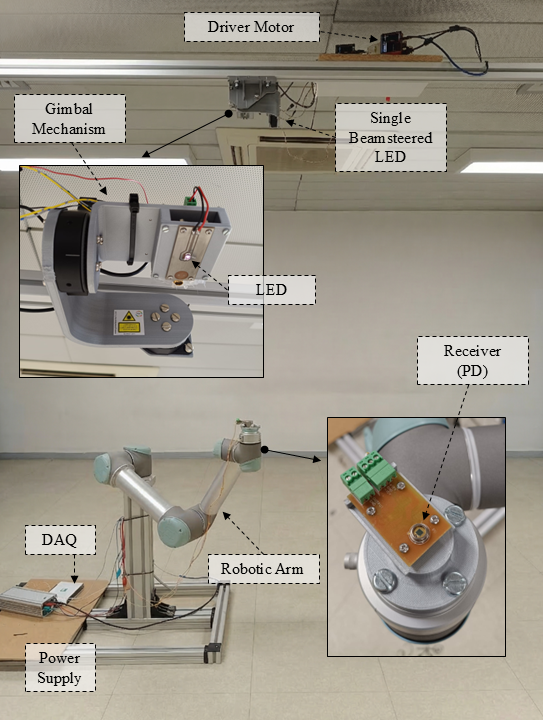
\includegraphics[width=0.85\linewidth]{figures/scheme.PNG}
    \caption{Photograph of the 3D robotic SBL-OWP testbed. 
    %The transmitter consists of a commercial IR LED mounted at the center of a two-axis motorized gimbal, while the receiver is a BPX61 PD front-end attached to the end-effector of a UR5 robotic arm for precise 3D positioning.
    }
    \label{fig:testbed_3d_setup}
\end{figure}

% -------------------------------------------------------
\subsection{Experimental Protocol for the SBL Method Evaluation}
\label{subsec:testbed_protocol}
% -------------------------------------------------------

For each receiver location, the measurement procedure was carried out as follows. First, the robotic arm placed the PD at the desired ground-truth 3D coordinate. Then, with the LED continuously turned on, the gimbal sequentially steered the transmitter toward $K=9$ predefined orientations found in \cite{acuna2025model} to be optimal for this SBL configuration. For each orientation, the DAQ recorded $10^3$ voltage samples, corresponding to $1~\mathrm{s}$ of observation time. The recorded voltage samples were stored as the raw RSS observations associated with the corresponding steering direction and 3D receiver position. This process was repeated for all selected points in the RoI, thereby generating the experimental database used in the subsequent analysis.

It is worth noting that the direction-finding stage based on the GLS and WLS estimators does not require the radiometric constant $C$ in \eqref{eq:C_constant_sbl}, since both estimators operate on inter-orientation RSS ratios. However, recovering the full 3D receiver position does require $C$, as described in \cite{acuna2025model}. Therefore, an initial calibration step was performed to estimate this constant. Specifically, the PD was positioned directly below the LED at known distances, with the LED pointing vertically downward and the PD pointing upward, so that the resulting RSS measurements could be substituted into \eqref{eq:sbl_lambertian} to solve for $C$. This procedure was repeated for receiver heights of $0.4$, $0.6$, $0.8$, $1.0$, and $1.2~\mathrm{m}$. The corresponding estimates were then averaged, yielding the value $C=6.2306$, which was subsequently used in the 3D position reconstruction stage.

% =======================================================
\section{Experimental Results and Discussion}
\label{sec:results}
% =======================================================


% -------------------------------------------------------
\subsection{SBL Method Validation and Estimator Comparison}
\label{subsec:sbl_validation_gls_wls}
% -------------------------------------------------------

Figure~\ref{fig:exp_3d_gls} shows the 3D distribution of the receiver position estimates obtained with GLS, with the color map representing the positioning error magnitude. The corresponding $x$--$y$ and $y$--$z$ projections are shown in Fig.~\ref{fig:exp_projections_gls}. The first and most important observation is that the SBL method works experimentally in 3D: throughout the measured RoI, the estimated points remain clustered around their corresponding ground-truth positions, despite relying on only one SBL and one simple PD. This confirms on real hardware the practical feasibility of the ratio-based SBL principle developed in Section~\ref{sec:system_model}.

Figures~\ref{fig:exp_3d_gls} and~\ref{fig:exp_projections_gls} also show that the error is not uniform but spatially structured, as the shortest ground-truth-to-estimate displacements are gathered around the center of the workspace, while larger deviations appear near the boundaries and corners. This trend is consistent with the geometry of the ratio construction. In the adopted steering set, the reference measurement $S_{1}$ corresponds to the nadir-pointing orientation. Hence, for peripheral receiver positions, the ratios $S_{k}/S_{1}$ involve a denominator acquired with a large off-axis irradiance angle. Since the LED datasheet specifies a semi-angle at half power of approximately $45^\circ$, the reference RSS becomes increasingly sensitive to deviations from the nominal Lambertian law as the receiver moves farther from the beam center. In turn, this sensitivity is propagated and amplified through the ratio-based hyperplane constraints, which explains why the largest errors are predominantly observed at the edges of the testbed.

Evaluation of the root mean square error (RMSE), mean absolute error (MAE), and of the 50th and 90th error percentiles (P50 and P90) enables to further characterize and compare the GLS and WLS estimators. As detailed in Table~\ref{tab:gls_wls_metrics}, GLS consistently outperforms WLS across all metrics, even though WLS provides a computational advantage, executing approximately 25\% faster than GLS \cite{acuna2025model}. This behavior is explicitly visualized in Fig.~\ref{fig:cdf_gls_vs_wls}, which shows the empirical cumulative distribution functions (CDF) of the 3D positioning error with both GSL and WLS, and highlights the better P50 and P90 performance of GLS. This performance difference is directly linked to the statistical structure of the SBL ratio model. As discussed in Section~\ref{subsec:gls_wls}, the empirical ratios are not only heteroscedastic but also mutually correlated because they share the same reference orientation. GLS explicitly incorporates the full covariance matrix of the ratio errors, whereas WLS retains only the diagonal weights and neglects cross-correlation terms. Consequently, both estimators behave similarly in favorable regions of the workspace, but GLS is more robust when the ratio reliability becomes uneven across orientations, e.g., for peripheral locations.

%This difference is also evident in Fig.~\ref{fig:cdf_gls_vs_wls}, where the GLS curve lies consistently to the left of the WLS curve and reaches the $90\%$ probability level at a substantially smaller error.

%Overall, these results establish the central experimental message of the paper: 3D positioning with a SBL is feasible in practice using a fully model-based closed-form estimator. Among the two estimators considered here, GLS provides the most accurate and robust performance.

\begin{figure}[tb]
    \centering
    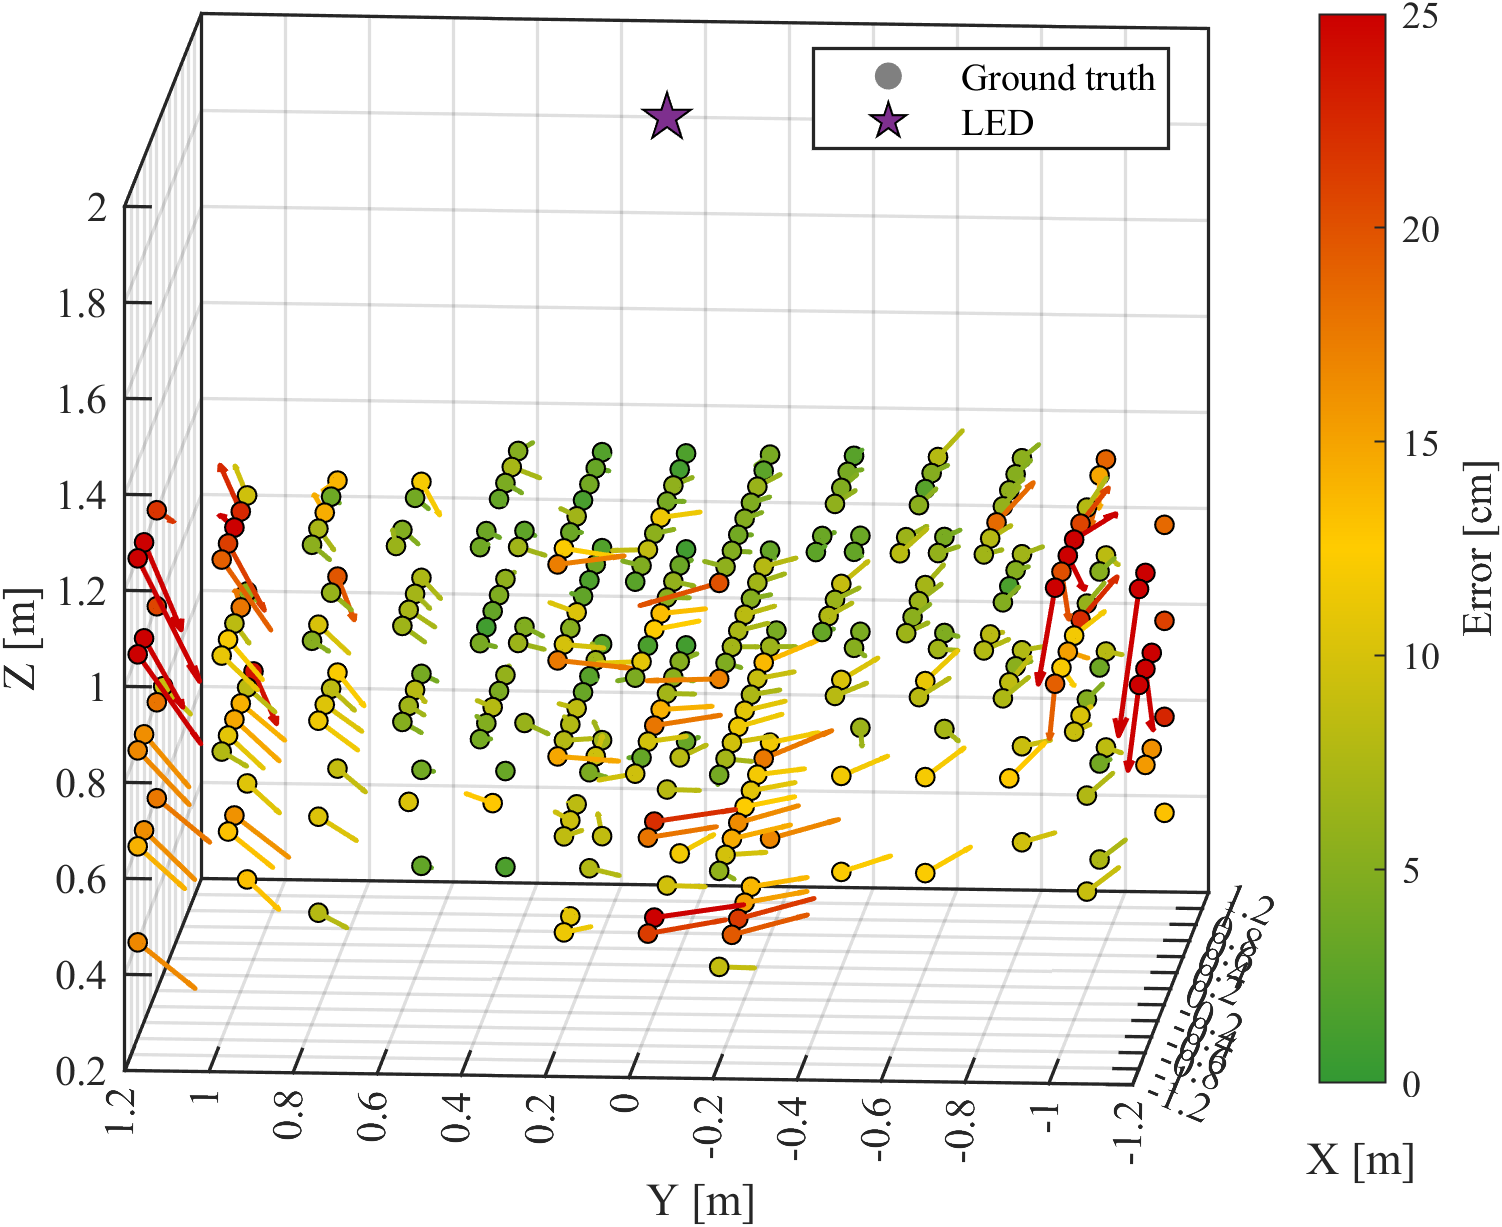
\includegraphics[width=\linewidth]{figures/Fig_3D_N9.png}
    \caption{Experimental 3D positioning results obtained with the GLS estimator for the $K=9$ SBL configuration. Ground-truth receiver positions are connected to their corresponding estimates, while the color map indicates the magnitude of the 3D positioning error.}
    \label{fig:exp_3d_gls}
\end{figure}

\begin{figure}[tb]
    \centering
    \subfloat[$x$--$y$ projection.]{%
        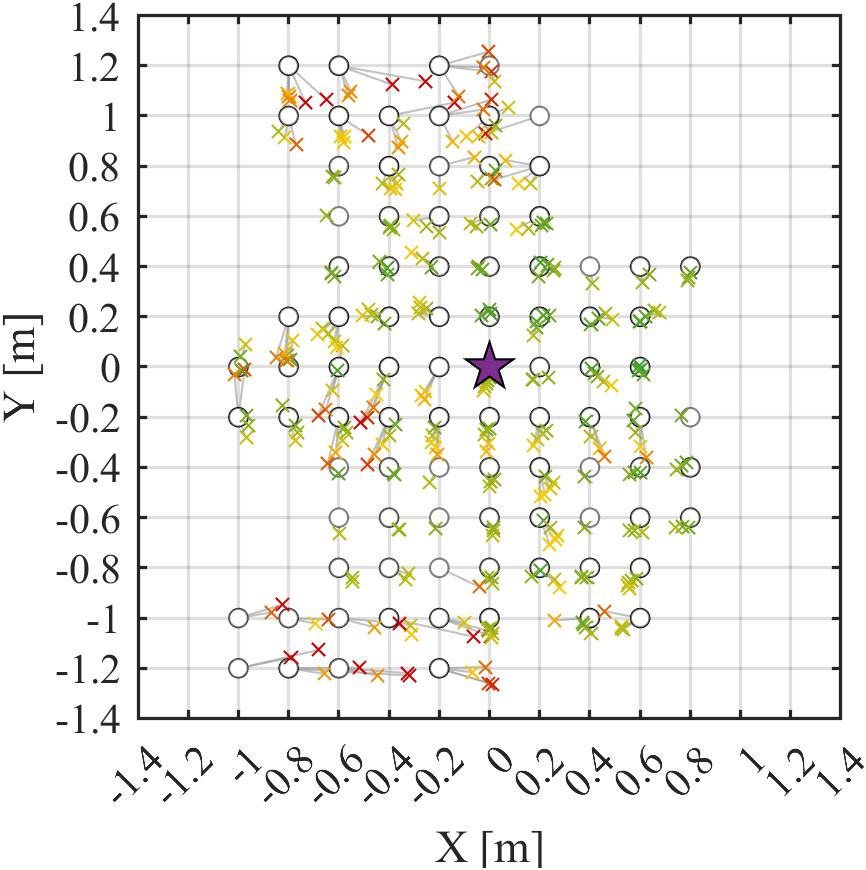
\includegraphics[width=0.48\linewidth]{figures/Fig_XY_N9.png}
        \label{fig:exp_xy_gls}
    }\hfill
    \subfloat[$y$--$z$ projection.]{%
        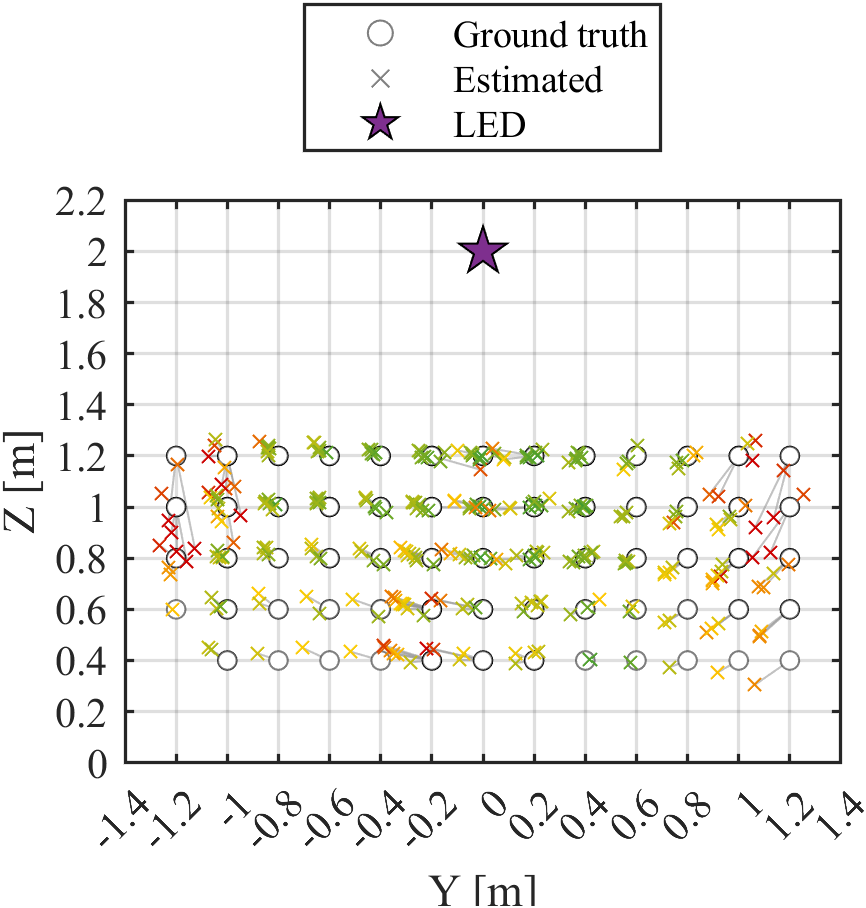
\includegraphics[width=0.46\linewidth]{figures/Fig_YZ_N9.png}
        \label{fig:exp_yz_gls}
    }
    \caption{Planar projections of the experimental localization results obtained with the GLS estimator for the $K=9$ SBL configuration. The line segments connect each ground-truth receiver position to its corresponding estimate. 
    %highlighting the spatial structure of the positioning error across the measured 3D region of interest.
    }
    \label{fig:exp_projections_gls}
\end{figure}

\begin{table}[tb]
\caption{Experimental comparison of the GLS and WLS estimators in terms of 3D position and pointing errors.}
\label{tab:gls_wls_metrics}
\centering
\setlength{\tabcolsep}{4pt}
\renewcommand{\arraystretch}{1.05}
\begin{tabular}{llcccc}
\hline
 & \textbf{Method} & \textbf{RMSE} & \textbf{MAE} & \textbf{P50} & \textbf{P90} \\
\hline
3D position error [cm] & GLS & $\mathbf{12.52}$ & 9.97 & 7.93 & 19.29 \\
                       & WLS & 15.79 & 11.98 & 8.56 & 27.04 \\
\hline
Pointing error [$^\circ$] & GLS & $\mathbf{4.87}$ & 4.06 & 3.36 & 7.66 \\
                     & WLS & 6.15 & 4.87 & 3.73 & 10.63 \\
\hline
\end{tabular}
\end{table}

\begin{figure}[tb]
    \centering
    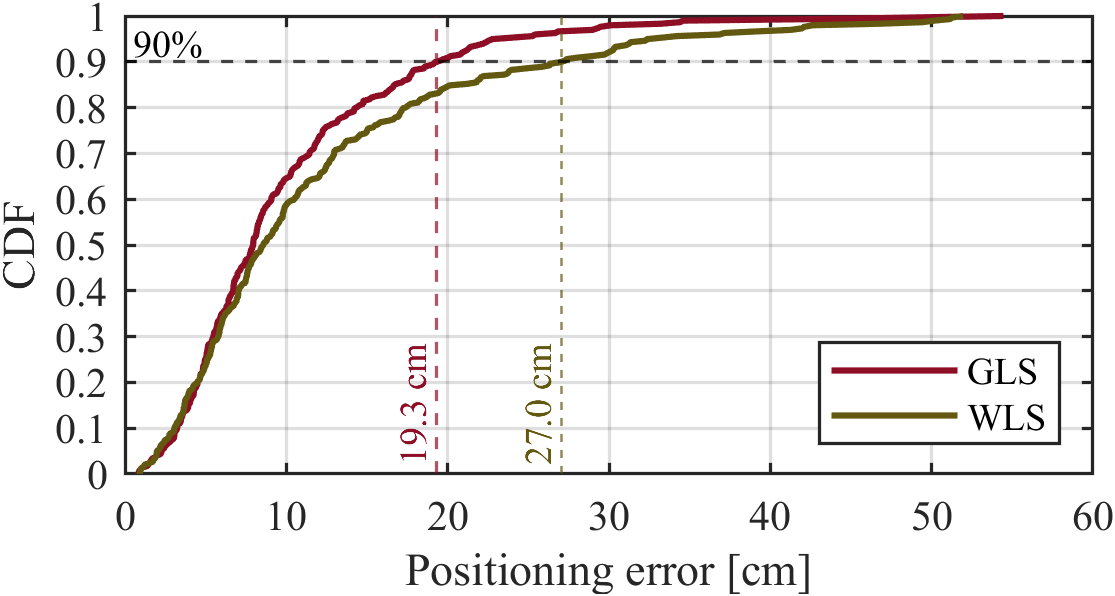
\includegraphics[width=0.9\linewidth]{figures/Fig_CDF_N9_GLS_vs_WLS.png}
    \caption{Empirical CDF of the 3D positioning error for the GLS and WLS estimators under the $K=9$ SBL configuration.}
    \label{fig:cdf_gls_vs_wls}
\end{figure}


% -------------------------------------------------------
\subsection{Direction Finding Performance}
\label{subsec:direction_finding_performance}
% -------------------------------------------------------

While the previous subsection assessed the SBL method in terms of full 3D positioning accuracy, for beam-steering applications the complete receiver position is not always required. In many practical OWC scenarios, estimating the LOS direction from the transmitter to the user is already sufficient to support beam alignment and establish a robust data link. For this reason, we now shift the focus from 3D position reconstruction to direction finding.

Let $\mathbf{n}_d$ and $\hat{\mathbf{n}}_d$ denote the ground-truth and estimated direction vectors, respectively. The direction-finding performance is quantified through the pointing error:
\begin{equation}
    \alpha = \arccos\!\left(\mathbf{n}_d^\top \hat{\mathbf{n}}_d\right).
    \label{eq:pointing_error}
\end{equation}
%The aggregate results are reported in Table~\ref{tab:gls_wls_metrics}. GLS again provides the best performance, with a pointing-error RMSE of $4.87^\circ$, and MAE of $4.06^\circ$. The corresponding WLS values are $6.15^\circ$, $4.87^\circ$. Thus, the superiority of GLS is preserved when the evaluation metric is changed from spatial position error to angular beam-pointing error.
The aggregate results are reported in Table~\ref{tab:gls_wls_metrics}. Consistent with the 3D positioning analysis, GLS yields the lowest pointing-error metrics, confirming that its superiority over WLS is firmly preserved when the evaluation metric is shifted from spatial position error to angular beam-pointing error.

This trend is clearly visible in Fig.~\ref{fig:cdf_pointing_error}, where the empirical CDF of $\alpha$ is shown for both estimators. The GLS curve lies consistently to the left of the WLS curve and reaches the $90\%$ probability level at a substantially smaller pointing error. From a beam-steering perspective, this is an important result: it shows that the experimentally validated SBL method not only localizes the receiver in 3D, but also estimates the steering direction with single-digit angular accuracy for most measured positions. Since the underlying application is transmitter-side beam alignment, this angular viewpoint is arguably more relevant than full position reconstruction.

To better understand the origin of the residual pointing errors, Fig.~\ref{fig:direction_finding}(a) plots $\alpha$ as a function of the ground-truth inclination $\theta$ of the receiver direction. Two regimes can be distinguished. For moderate inclinations, both estimators remain relatively accurate and the pointing error stays low. However, once $\theta$ exceeds approximately $40^\circ$--$45^\circ$, the error starts to increase, and the increase is markedly stronger for WLS than for GLS. This behavior is consistent with the ratio-based formulation, since more oblique directions are associated with weaker and less balanced inter-orientation RSS measurements, making the direction estimate more sensitive to model mismatch and ratio uncertainty.

%Further insight is provided by Figs.~\ref{fig:direction_finding}(b) and \ref{fig:direction_finding}(c), which compare the estimated and ground-truth spherical angles of the receiver direction. Fig.~\ref{fig:direction_finding}(b) shows that the main difference between GLS and WLS lies in the inclination estimate. Up to moderate inclination values, both estimators follow the ideal diagonal reasonably well. At larger inclinations, however, the WLS estimates exhibit a stronger systematic deviation and a wider spread, with many samples departing noticeably from the $\pm5^\circ$ band. In contrast, GLS remains more tightly clustered around the ideal trend, although some bias is still observed at the largest angles. This visual observation is confirmed quantitatively: the inclination RMSE/MAE are $3.29^\circ/2.54^\circ$ for GLS and $4.68^\circ/3.51^\circ$ for WLS. Hence, the main source of the performance gap in pointing error is the improved inclination recovery provided by GLS.

Further insight is provided by Figs.~\ref{fig:direction_finding}(b) and \ref{fig:direction_finding}(c), which compare the estimated and ground-truth spherical angles of the receiver direction. For any estimated unit direction vector $\hat{\mathbf{n}}_d = [\hat{n}_{x}, \hat{n}_{y}, \hat{n}_{z}]^\top$, these angular coordinates are analytically extracted as $\hat{\theta} = \arccos(-\hat{n}_{z})$---defining the inclination relative to the downward vertical axis---and $\hat{\varphi} = \mathrm{atan2}(\hat{n}_{y}, \hat{n}_{x})$ for the azimuth. Fig.~\ref{fig:direction_finding}(b) shows that the main difference between GLS and WLS lies in the inclination estimate. Up to moderate inclination values, both estimators follow the ideal diagonal reasonably well. At larger inclinations, however, the WLS estimates exhibit a stronger systematic deviation and a wider spread, with many samples departing noticeably from the $\pm5^\circ$ band. In contrast, GLS remains more tightly clustered around the ideal trend, although some bias is still observed at the largest angles. This visual observation is confirmed quantitatively: the inclination RMSE/MAE are $3.29^\circ/2.54^\circ$ for GLS and $4.68^\circ/3.51^\circ$ for WLS. Hence, the main source of the performance gap in pointing error is the improved inclination recovery provided by GLS.



By contrast, Fig.~\ref{fig:direction_finding}(c) shows that the azimuth estimate is accurate for both estimators over almost the entire angular range. Most samples remain close to the ideal diagonal and within the $\pm10^\circ$ band, with only minor differences between GLS and WLS. This is again supported by the numerical results, since the azimuth RMSE/MAE are $6.88^\circ/5.06^\circ$ for GLS and $6.94^\circ/5.07^\circ$ for WLS. Therefore, the dominant contribution to the overall pointing-error difference does not come from azimuth estimation, but from inclination estimation under increasingly oblique geometries.

%\textcolor{red}{Overall, these results show that the proposed SBL method is experimentally effective not only for 3D localization, but also for direct beam-pointing purposes. In that context, direction finding emerges as a particularly meaningful performance metric, and the comparison confirms that GLS provides the most reliable angular estimates, especially in the challenging off-axis regime.}

\begin{figure}[tb]
    \centering
    \includegraphics[width=\linewidth]{figures/Fig_CDF_pointing_error.png}
    \caption{Empirical CDF of the pointing error for the GLS and WLS estimators. The pointing error is defined as the angular difference between the estimated and true direction of the LED.}
    \label{fig:cdf_pointing_error}
\end{figure}


\begin{figure*}[tb]
    \centering
    \raisebox{0.5cm}{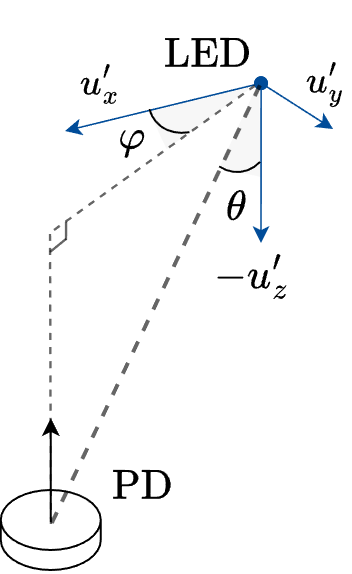
\includegraphics[width=0.12\textwidth]{figures/Fig_apoyo.png}}
    \label{fig:apoyo}
    \hfill
    \subfloat[]{%
        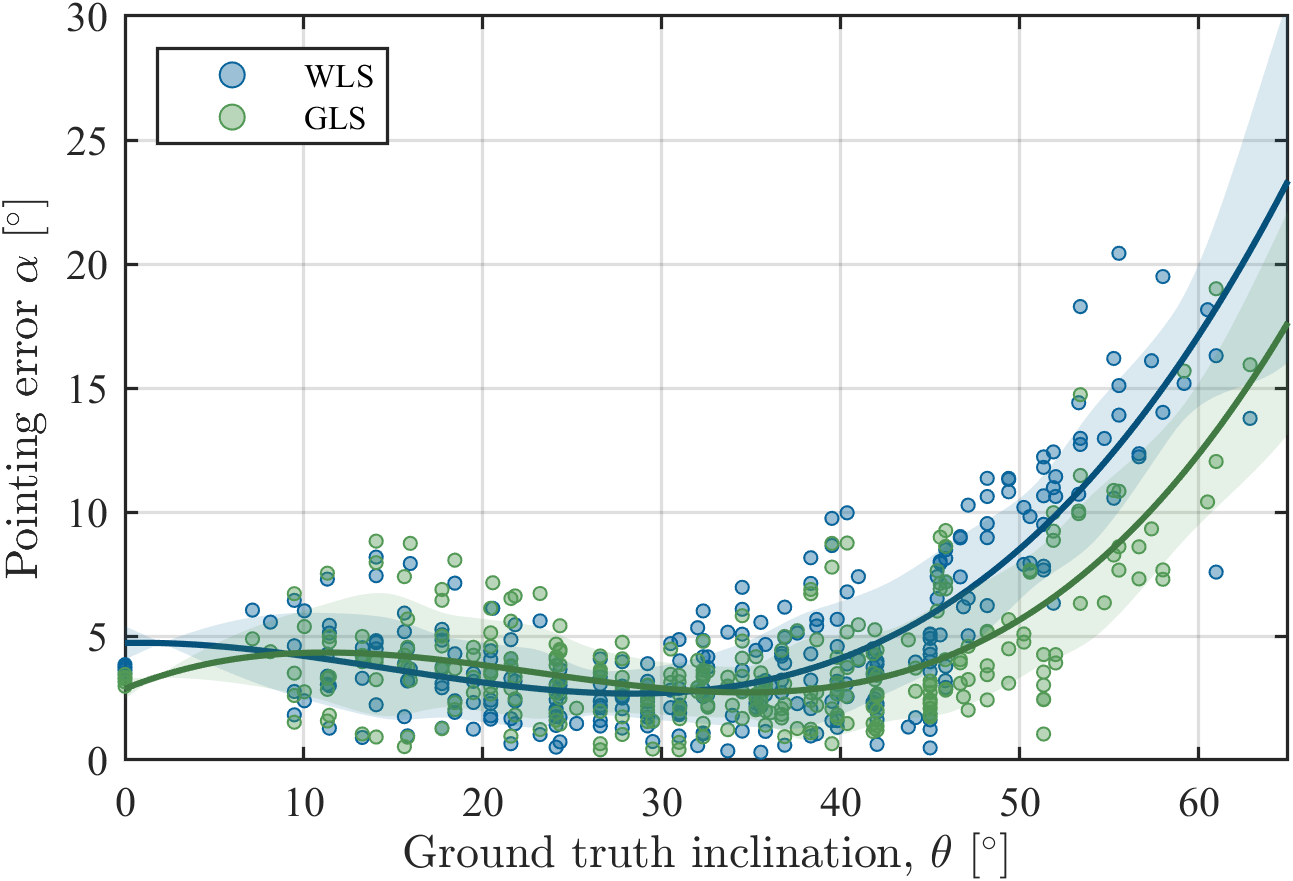
\includegraphics[width=0.35\textwidth]{figures/Fig_error_vs_offaxis.png}
        \label{fig:direction_error_vs_offaxis}
    }\hfill
    \subfloat[]{%
        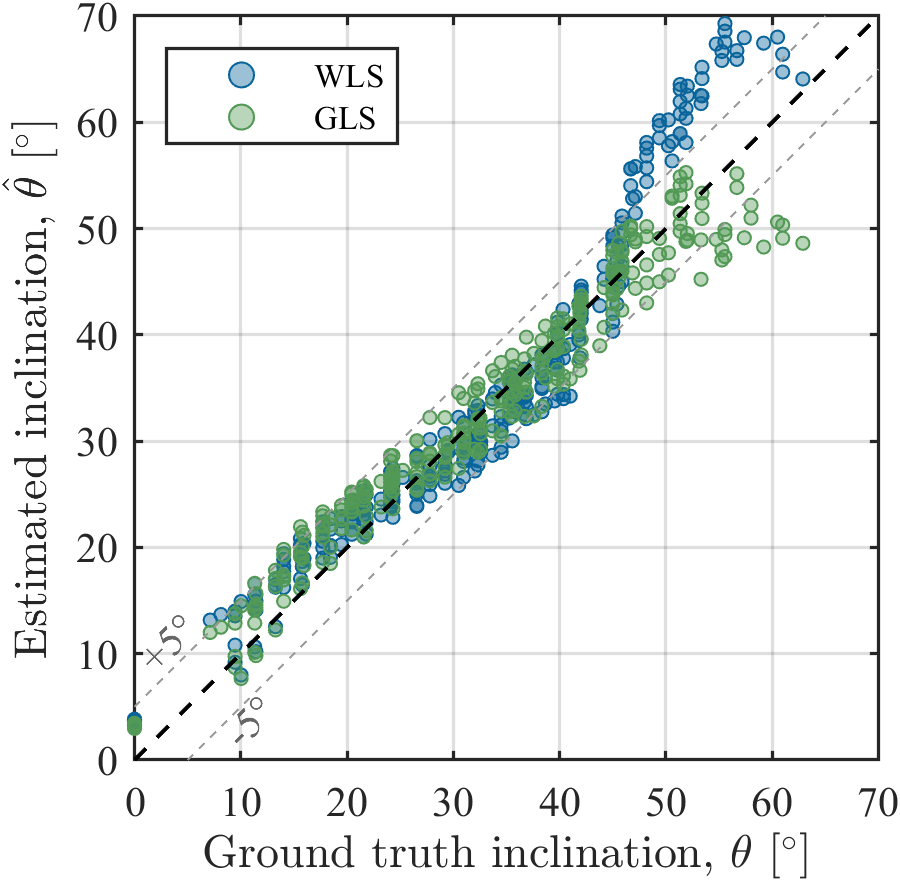
\includegraphics[width=0.24\textwidth]{figures/Fig_inclination.png}
        \label{fig:direction_inclination}
    }\hfill
    \subfloat[]{%
        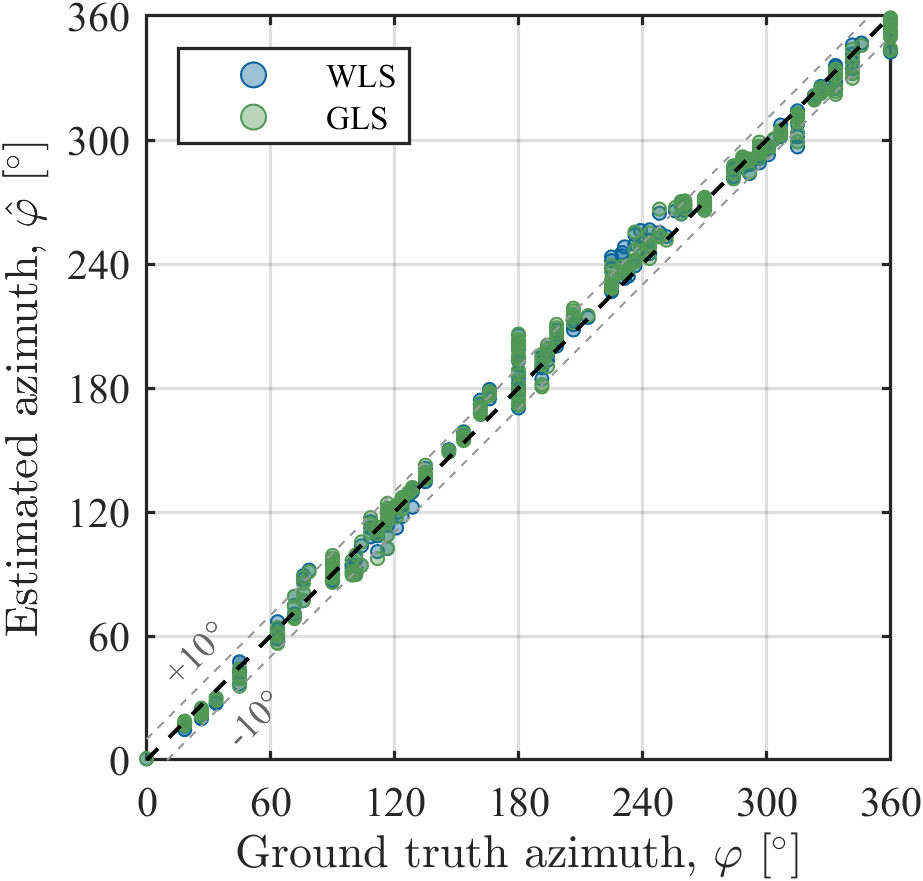
\includegraphics[width=0.25\textwidth]{figures/Fig_azimuth.png}
        \label{fig:direction_azimuth}
    }
    \caption{Direction finding performance of the GLS and WLS estimators: (a) pointing errors, (b) inclination error, and (c) azimuth error.}
    \label{fig:direction_finding}
\end{figure*}
%0.4, 0.28, 0.29




% -------------------------------------------------------
\subsection{Position Estimation Stability}
\label{subsec:position_estimation_stability}
% -------------------------------------------------------
{\color{blue}
Having established GLS as the most reliable estimator, we now examine the stability of the 3D position estimate as a function of the RSS integration time. Figure~\ref{fig:position_stability_boxplot} reports boxplots of the 3D positioning error for three representative transmitter--receiver distances, namely $\|\mathbf{d}\|=0.80~\mathrm{m}$, $1.36~\mathrm{m}$, and $2.15~\mathrm{m}$. 
This analysis is practically relevant because the integration time directly determines the acquisition latency per steering orientation and, therefore, the overall update rate of the SBL system. Since the DAQ operates at $1~\mathrm{kHz}$, an integration window of $T_{\mathrm{int}}$ ms is equivalent to averaging $N=T_{\mathrm{int}}$ samples per orientation.

Statistically, the median positioning error remains essentially unchanged as the integration time increases. By contrast, the dispersion of the error distribution decreases with $T_{\mathrm{int}}$, as reflected by the narrowing interquartile range and the reduction of outliers. This effect is weak at $\|\mathbf{d}\|=0.80~\mathrm{m}$, more noticeable at $\|\mathbf{d}\|=1.36~\mathrm{m}$, and clearly pronounced at $\|\mathbf{d}\|=2.15~\mathrm{m}$, where the interquartile range decreases from $0.610~\mathrm{cm}$ at $1~\mathrm{ms}$ to $0.127~\mathrm{cm}$ at $50~\mathrm{ms}$.
Therefore, the benefit of longer integration is limited at short distances and becomes increasingly relevant as the link distance grows.

These results indicate that increasing the integration time mainly improves repeatability rather than absolute accuracy. Temporal averaging reduces variability, but it does not significantly modify the central error level at a given location, which suggests that the absolute positioning error is dominated by systematic effects rather than by short-term measurement noise. In the present setup, these systematic effects are primarily associated with hardware nonidealities and model mismatch, in particular the quasi-Lambertian and asymmetric radiation profile of the commercial LED. From a system-design perspective, this is an important result: the proposed method does not require long acquisition windows to preserve its localization performance. In practice, an integration time around $20~\mathrm{ms}$ already provides a favorable trade-off, since it yields a substantial reduction in dispersion compared with very short windows while remaining close to the plateau reached at longer averaging times.
}

\begin{figure}[tb]
    \centering
    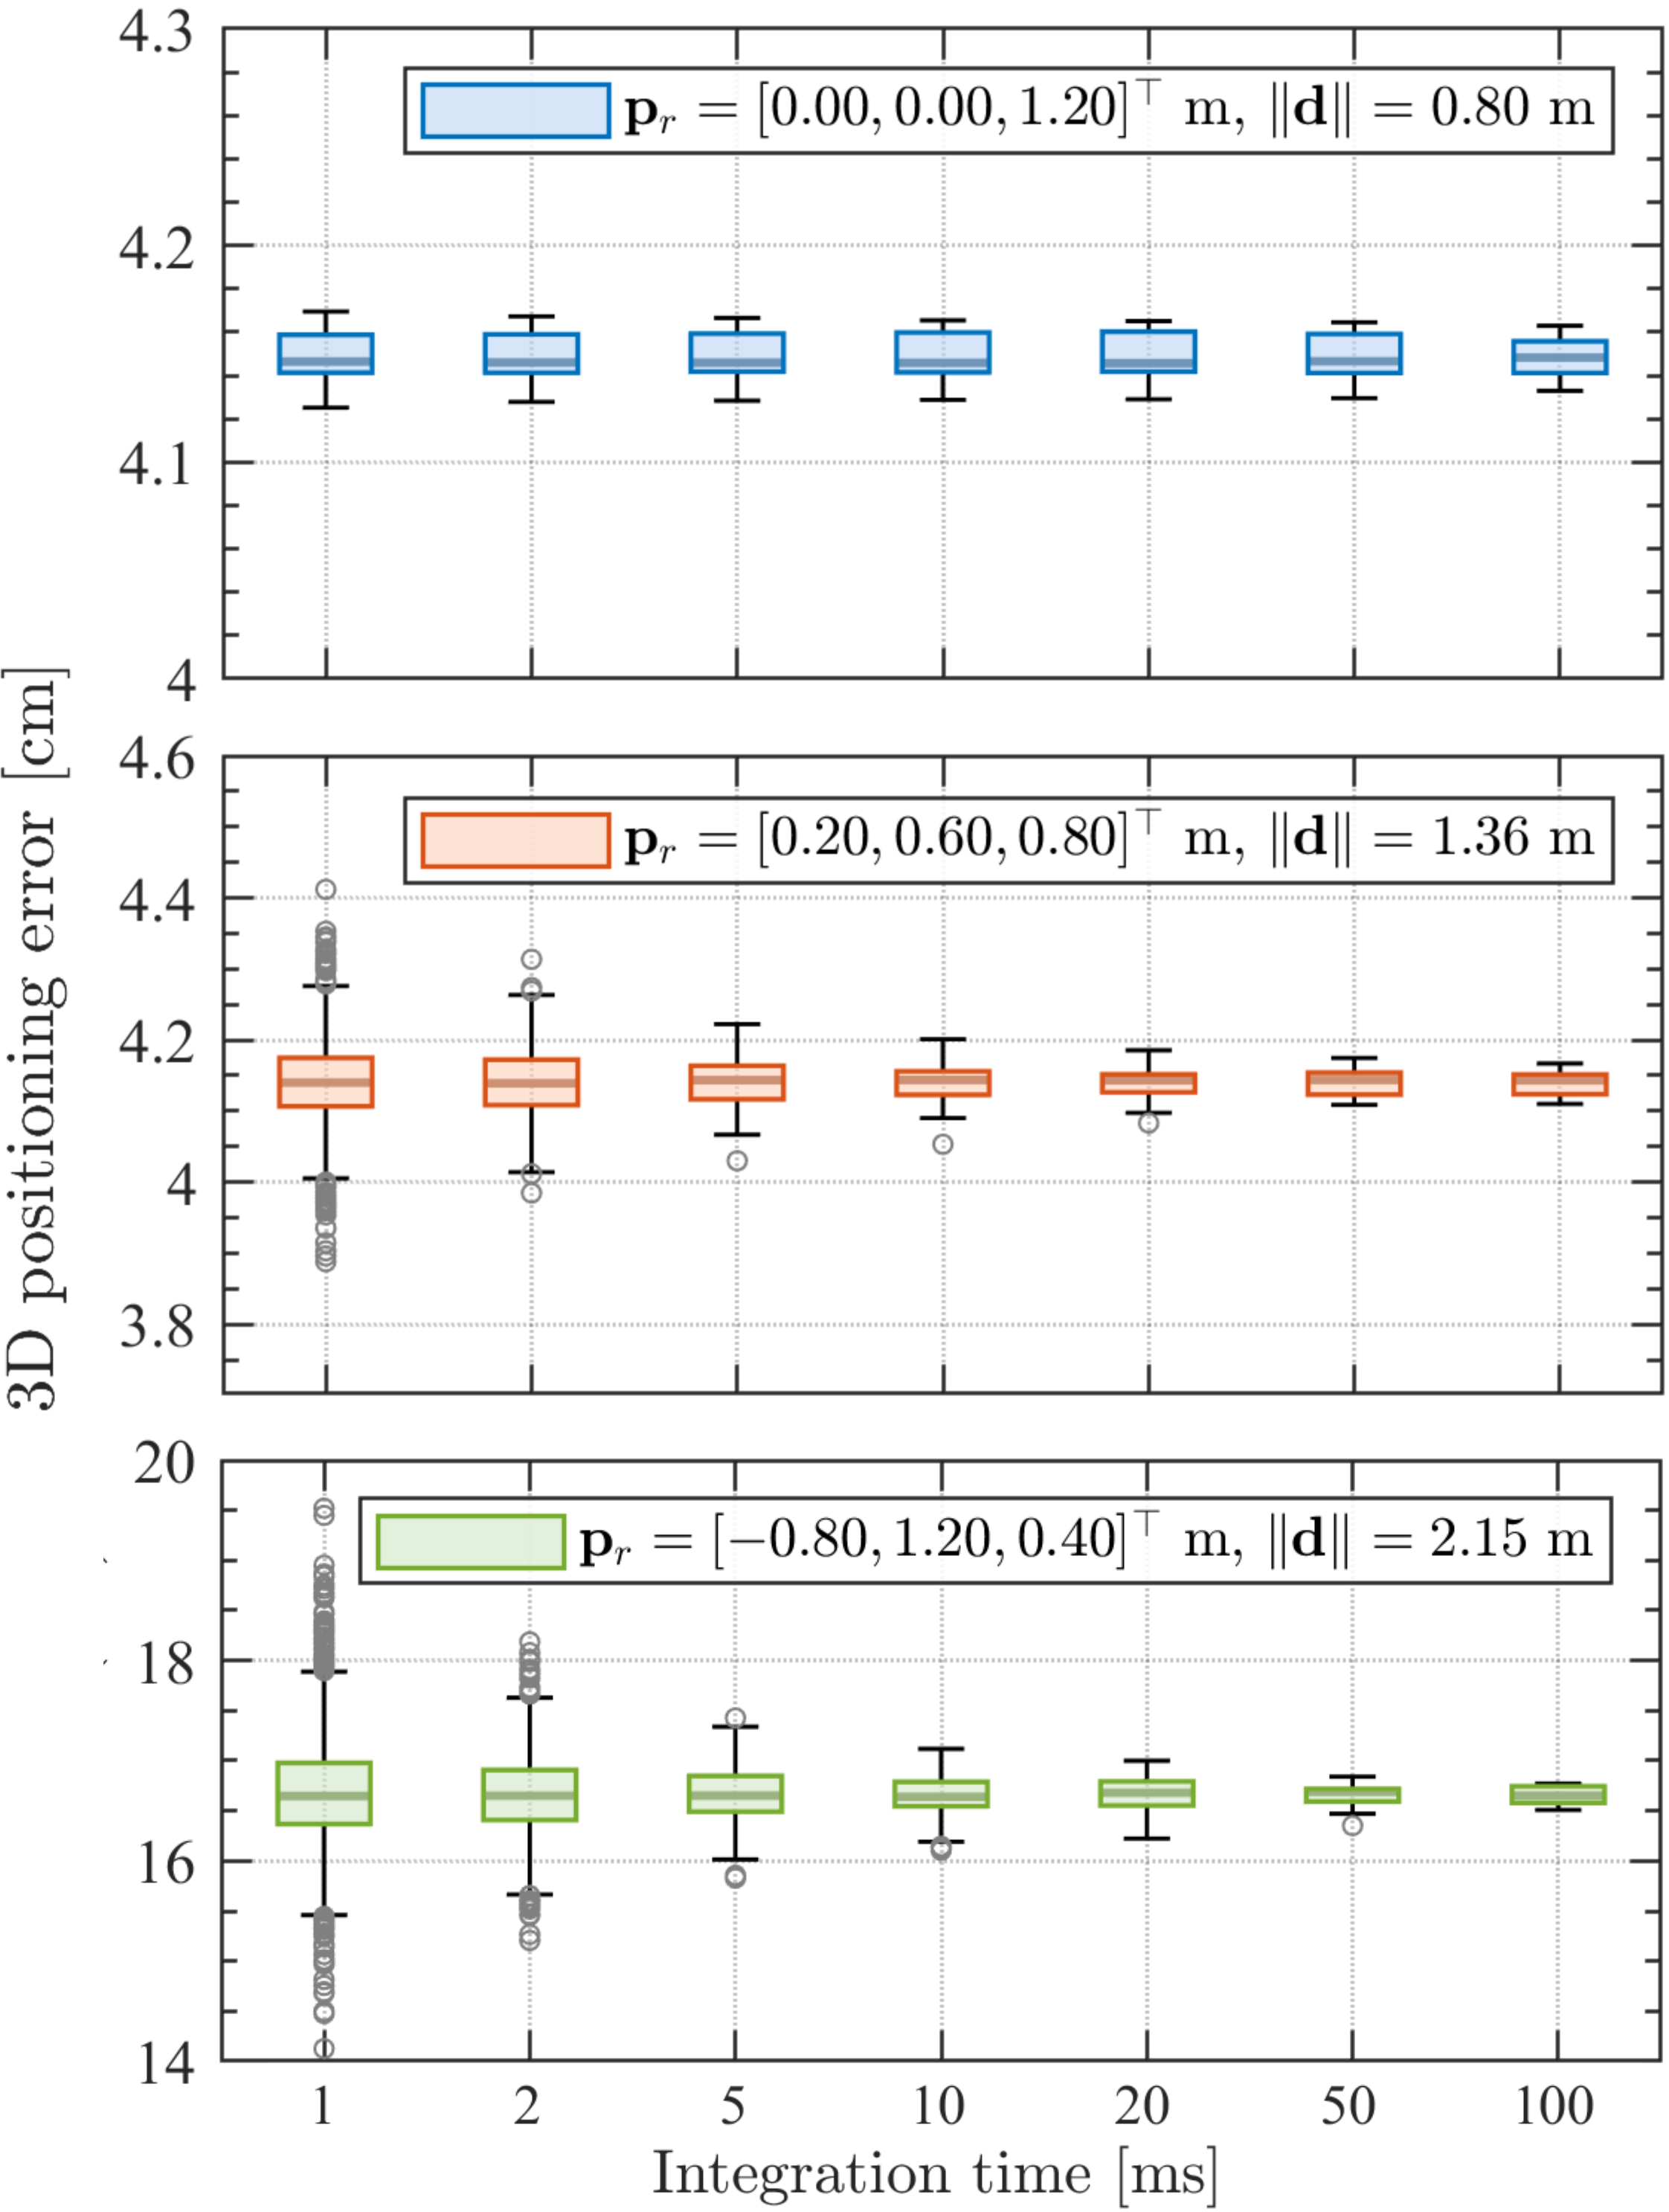
\includegraphics[width=0.9\linewidth]{figures/Fig_distribution.png}
    \caption{Boxplot-based analysis of the 3D positioning error obtained with the GLS estimator for three representative receiver locations at different transmitter--receiver distances.}
    \label{fig:position_stability_boxplot}
\end{figure}


% =======================================================
\section{Conclusions}
\label{sec:conclusions}
% =======================================================

This paper presented the first experimental validation of 3D OWP based on a SBL and a single PD receiver. Building on the ratio-based SBL formulation previously derived in \cite{acuna2025model}, the study demonstrated that a fully model-based closed-form approach remains experimentally viable in a real robotic testbed while keeping the receiver architecture extremely simple and concentrating the steering complexity at the infrastructure side. The results showed that the method is effective not only for full 3D localization, but also for direction finding, which is particularly relevant for beam-steering operation in OWC.

Among the two estimators considered, GLS consistently outperformed WLS in both spatial and angular performance. For 3D positioning, GLS reduced the MAE from $11.98~\mathrm{cm}$ to $9.97~\mathrm{cm}$. For direction finding, GLS achieved a pointing-error MAE of $4.06^\circ$, confirming its superior robustness, especially at large off-axis inclinations. 
\textcolor{blue} {In addition, the integration-time analysis showed that the median positioning error remains essentially stable over a wide range of averaging windows, whereas the dispersion of the error distribution decreases with temporal averaging, especially at larger transmitter--receiver distances.}
Overall, these results validate the practical feasibility of single-LED 3D OWP and support its relevance for future indoor localization and beam-aware optical wireless systems. Future work will focus on mitigating the residual spatial biases caused by the quasi-Lambertian asymmetry of commercial LEDs by incorporating empirical radiation maps into the estimation framework.


\section*{Acknowledgment} This work was supported by the European Union's Smart Networks and Services Joint Undertaking (SNS JU) under grant agreement `OPTI-6G' No. 101139292.



\bibliographystyle{IEEEtran}
\bibliography{OWP}

\end{document}
